\documentclass[titlepage]{article}
\usepackage[left=15mm,right=15mm,top=1in,bottom=1in]{geometry}
\usepackage{framed}
\usepackage{caption}
\usepackage{amsmath}
\usepackage{hyperref}
\usepackage{imakeidx}
\usepackage{graphicx}
\usepackage{array}

\newcolumntype{C}[1]{>{\centering\arraybackslash} m{#1cm}}
\graphicspath{{./img/}}

\makeindex

\title{Autonomous Pool Playing Robot\\~\\\textbf{\Huge{Hardware Design}}}
\author{
	Ernest Selman\\selmae@mcmaster.ca\\1201291\\~\\\and
	Guy Meyer\\meyerg@mcmaster.ca\\1320231\\~\\\and
	Eric Le Fort\\leforte@mcmaster.ca\\1308609\\~\\\and
	Andrew Danha\\danhaas@mcmaster.ca\\1223881\\~\\\and
	Derek Savery\\saverydj@mcmaster.ca\\1219142\\~\\
}
 
\begin{document}
\maketitle
\tableofcontents
\listoftables
\listoffigures

\vfill
\begin{table}[!htbp]
\centering
\begin{tabular}{| C{3} | C{2} | C{5} | C{2.5} |}\hline
	Date		&Revision \#	&Comments	&Authors\\\hline
	6/12/2016	&0	&- Document initialized		&Eric Le Fort\\\hline
	7/12/2016	&0	&- First draft completion	&Guy Meyer\newline Ernest Selman\newline Derek Savery\newline Andrew Danha\newline Eric Le Fort\\\hline
	20/03/2017	&1	&- Consolidated design document creation	&Eric Le Fort\\\hline
	25/03/2017	&1	&- Updated Mechanical and Electromechanical sections	&Guy Meyer\\\hline
	25/03/2017	&1	&- Updated Electrical section	&Derek Savery\newline Andrew Danha\\\hline
	26/03/2017	&1	&- Revision 1 completion	&Eric Le Fort\\\hline
\end{tabular}
\caption{Revision History}
\end{table}
\clearpage

\section{Introduction}
This document will fully describe the hardware design of the Autonomous Pool Playing Robot. This document is intended to prepare the hardware team for construction/ordering of each component discussed within as well of construction of the final product.
\subsection{System Description}
The hardware part of this system will consist of the mechanical, electromechanical, and electrical subsystems which in combination will form the autonomous pool playing robot.\\\\
The mechanical components will form the structure of the robot in order to allow the end effector to move in the X, Y, and Z axis, rotate about the Z axis, and provide the support to maintain the stability of the system. The electromechanical components will facilitate motion of the robot including actuating the end-effector. The electrical components will power the entire system as well as deliver signals to the electromechanical devices in order to drive the motion of the robot.
\subsection{Overview}
This document has four sections not including this one. Each section will describe the high level design of the subsystem as well as the various components which make up that subsystem. The three subsystems and components will be illustrated using a combination of CAD models, diagrams, and various descriptive characteristics such as lists of requirements that must be met by the specific components.\\
\begin{itemize}
	%\item \textbf{Parts List}: This section will list all parts required to create this system as designed.\\
	\item \textbf{Mechanical Subsystem}: This section will define the mechanical aspect of this system.\\
	\item \textbf{Electromechanical Subsystem}: This section will define the electromechanical aspect of this system.\\
	\item \textbf{Electrical Subsystem}: This section will define the electrical aspect of this system.\\
	\item \textbf{Construction}: This section will describe the process by which to construct this system as well as any equipment or tools that will be needed.\\
\end{itemize}
\newpage
\subsection{Naming Conventions \& Definitions}
This section outlines the various definitions, acronyms and abbreviations that will be used throughout this document in order to familiarize the reader prior to reading.
\subsubsection{Definitions}
Table \ref{tab:Definitions} lists the definitions used in this document. The definitions given below are specific to this document and may not be identical to definitions of these terms in common use. The purpose of this section is to assist the user in understanding the requirements for the system.
\begin{table}[h!]
\centering
\caption{Definitions}
\begin{tabular}{| C{6} | p{6cm} |}\hline
	\textbf{Term}	&\textbf{\centering Meaning}\\\hline
	X-axis					&Distance along the length of the pool table\\\hline
	Y-axis					&Distance across the width of the pool table\\\hline
	Z-axis					&Height above the pool table\\\hline
	End-effector			&The end of the arm that will strike the cue ball\\\hline
	$\theta$				&Rotational angle of the end-effector\\\hline
	Cue 					&End-effector\\\hline
	Personal Computer		&A laptop that will be used to run the more involved computational tasks such as visual recognition and the shot selection algorithm\\\hline
	Camera					&Some form of image capture device (e.g. a digital camera, smartphone with a camera, etc.)\\\hline
	Table State				&The current positions of all the balls on the table\\\hline
	Entity					&Classes that have a state, behaviour and identity (e.g. Book, Car, Person, etc.)\\\hline
	Boundary				&Classes that interact with users or external systems\\\hline
\end{tabular}
\label{tab:Definitions}
\end{table}

\subsubsection{Acronyms \& Abbreviations}
Table \ref{tab:Acronyms} lists the acronyms and abbreviations used in this document.
\begin{table}[h!]
\centering
\caption{Acronyms and Abbreviations}
\begin{tabular}{| p{6cm} | p{6cm} |}\hline
	\textbf{Acronym/Abbreviation}	&\textbf{Meaning}\\\hline
	VR								&Visual Recognition\\\hline
	PC								&Personal Computer\\\hline
	$\mu$C							&Micro-Controller\\\hline
	EE								&End-Effector\\\hline
	EEB								&End-Effector Base\\\hline
	EEA								&End-Effector Arm\\\hline
	PWM								&Pulse Width Modulation\\\hline
	I/O								&Input/Output\\\hline
\end{tabular}
\label{tab:Acronyms}
\end{table}
\newpage



%\section{Parts List}



\section{Mechanical System}
This section will go into further detail regarding each mechanical component that is to be designed as part of this system.

% DONE 	TODO: Just need Overall - Full Picture
\subsection{X-Rails}
\textbf{Description}\\
The X-rails are the largest source of translational motion in the system. They are responsible for carrying the rest of the system along the length of the table. The motion will be induced by two motors that apply power from the end of this axis (details of motor type and specification is described in the electrical section of this document). Both sides of the table will be equipped with an X-rail since it will carry most of the load and that will provide greater stability in an evenly distributed manner. The motion of the X-rail is synchronous, meaning that both sides will follow the same commands and actuate together.\\\\
\textbf{Requirements}\\
The X-rails will be required to run the full length of the pool table. Furthermore, they will be required to support the full weight of the rest of the mechanical components by transferring it to the sides of the pool table.
\begin{center}
	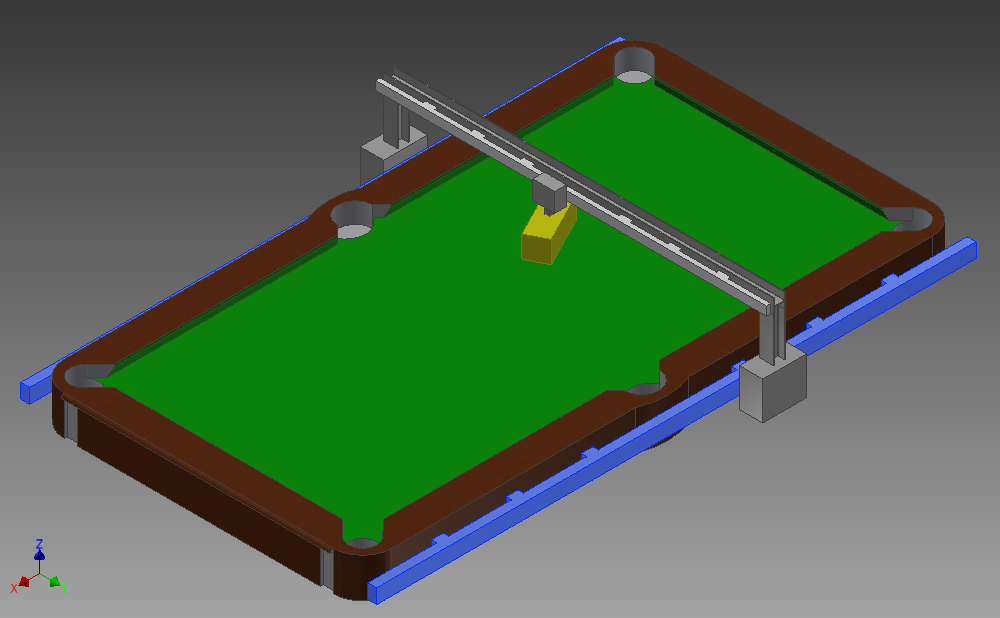
\includegraphics[width = 0.9\textwidth]{xRails1.png}	% TODO: Include new picture
\captionof{figure}{X-Rails relative to the table (found in blue) }
\label{fig:xRailFig}
\end{center}

\newpage
\subsection{Metal X Rail}
\textbf{Description}\\
The X Rails are the longest part of the system and provide structural support for the entire system. They are attached along the length of the table with long bolts to allow clearance for the shooting mechanism (with improvements in the Shooting Mechanism the rail may be brought closer to the table to minimize its footprint). The material used for these rails is hot rolled steel and purchased to be as straight as possible.\\\\
\textbf{Requirements}\\
This component must be optimized to reduce its footprint as much as possible. To allow smooth motion in the x direction, the rail must be straight and consistent in width as to not force the Arm Base to encounter bumps. With different shooting mechanisms the rail may be adjusted in length and distance from the table. The holes in the rail are responsible for 4 tasks; attaching to the side of the table with 6 long rod connections, supporting the NEMA 23 motor holder on on end, supporting the x-rail pulley on other end, and supporting the Arm Base which attaches to the rest of the system.

\subsection{NEMA 23 Motor Holder}
\textbf{Description}\\
The NEMA 23 Motor Holder is used to mount the NEMA 23 motor to the X Rail. By providing 4 bolt attachment for the motor and 2 bolt attachment for the rail, the NEMA 23 can be placed at a proper height as to apply sufficient force to the Arm belt connector. The holder is machined out of PVC which has strong structural features and is easy to work with. To reduce vibrational noise from the motor it is recommended to place soft, absorbing element between the holder and the X-Rail.\\\\
\textbf{Requirements}\\
This component is required to holder the motor with a rigid grip. It is highly recommended to tighten all connections to avoid jitter while the motor is running (this ensures consistency and accuracy). The height of the motor is dependant on the height of the belt holder attached to the Arm. This desired height can be estimated by analyzing the centre of mass of the system and placing the motor along that axis. 

%TODO: include pulley holder exploded pic from X Rail folder
\subsection{X Rail Pulley Holder - Rail Attachment}
\textbf{Description}\\
The Rail Attachment (labeled P1 in exploded view) is used to couple the X Rail to the linear motion which tightens the belt. Its simple L shape provides sufficient thickness for bolts B1 and B2 which connect to the X Rail and for B3 which attaches to P2. \\\\
\textbf{Requirements}\\
This component must not interfere with the motion of the belt while providing sufficient strength even for high tensions.

\subsection{X Rail Pulley Holder - Pulley Attachment}
\textbf{Description}\\
The Pulley Attachment (labeled P2 in exploded view) is used to hold the idle pulley responsible for supporting the timing belt of the X Rail. As the N2 wing nut is turned it will pull on B3 which moves P2 away from the motor, this results in tightening.\\\\
\textbf{Requirements}\\
This component must not interfere with the rotation of the pulley or the motion of th belt as it interacts with this assembly. Bolt B4 must be long enough to be bolted on the opposite side. 

\newpage
\subsection{Table-Rail Rod Connections}
\textbf{Description}\\
The Table-Rail Rod Connections are a set of 6x 11 inch rods used to hold the X Rail sufficiently far from the table. The Adjustment of their length can be optimized to ensure that the rail is as close to the table as possible.\\\\
\textbf{Requirements}\\
This component must not interfere with the linear motion of the Arm Base. They must be tightened to the table so that they are as perpendicular as possible (This ensures that the Y Rail is straight as well).

\subsection{Timing Belt}
\textbf{Description}\\
The Timing Belt travels along the entire length of the table twice to connect to both side of the belt holder (attached to Arm), wrap around driver pulley of the motor and the idoler pulley in the pulley holder assembly.\\\\
\textbf{Requirements}\\
This bet must be rigid and low in flexibility. When tightened it should grip the idler and the driver pulley well without slip. Please note that excessive tightening may cause unwanted friction in the wheels of the Arm Base and/or unwanted tension on the belt itself and its connecting components.

\subsection{Supporting Wood}
\textbf{Description}\\
Supporting wood may be added to the sides for the table where the rod connections are made which helps provide perpendicular support to the rods. This reduces the stress on table and may help over time. Note that its addition is subjective to table conditions and may be unnecessary.
\\~\\
\textbf{Requirements}\\
The Wood must not interfere with the motion of the rail or obstruct the system in any way. Not further requirements or restrictions are mandated.

% TODO: NEED TO ADD NEMA 17 Motor holder and pulley holder
% TODO: Just need Overall -Y Rail  Full Picture
\newpage
\subsection{Y-Rails}
\textbf{Description}\\
The Y-rail allows for translational motion of the End Effector along the width of the table. The support for this component will be provided via L-shaped brackets in the Arms. The rails are composed of aluminum and are chosen with their angled shape to counteract the bending which may occur in long metal bars with a moving load.
\\~\\
\textbf{Requirements}\\
The purpose of the Y-rail is to provide motion of the end-effector base in the Y-axis with low friction. It must allow traversal of the entire width of the table smoothly. It is not a requirement to support the EE since that will be done by the bridge, although these components may become one if the Y-rail is strong enough on its own.
\begin{center}
	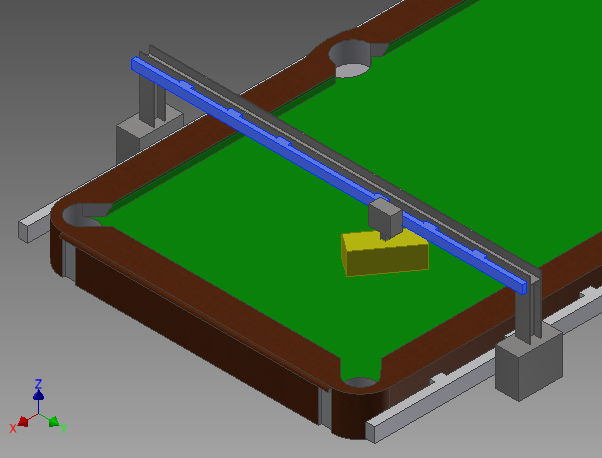
\includegraphics[width = 0.9\textwidth]{yRail1.png} 		% TODO: Include new picture
\captionof{figure}{Y Rail relative to the table (found in blue) }
\label{fig:yRailFig}
\end{center}

\subsection{Bolt Connections to Y Rail}
\textbf{Description}\\
In order to connect the Y Rail to the Arm there is a bolt connection to the L-shaped brackets located at the top of the Arm structure. Two bolts are used to connect the Y Rail to the bracket in order to reduce the swinging in the y-direction. It is recommended to tighten the bolts after correct positioning of the Y Rail.\\\\
\textbf{Requirements}\\
This component is required to be strong enough to support the Y Rail but also not to interfere with other bolts in the system.

% Complete: Section rewritten and updated (only needs pictures) <- TODO
\newpage
\subsection{Camera Mount}
\textbf{Description}\\
The camera mount is the component that holds the device responsible for image capture to be used by the VR. The camera mount is a simply phone holder that connects to the ceiling with the help of 4x 1-1/2" bolts along with nuts on opposite side. The fragile ceiling tile is replaced with a sturdy sheet of white plywood with holes in order to perfectly place the phone where most comfortable. The phone location may also be adjusted by removing the ceiling tile and unscrewing the holder. Ideally once the phone holder is connected it will remain in that position since the pool table should not move.\\~\\
\textbf{Requirements}\\
The camera mount is required to ensure that the mobile device is located sufficiently high and parallel to the table. This is to allow the VR software to be able to consistently analyze the image with accuracy. It is vital that the structure does not interfere with any of the moving mechanical components present. Furthermore, it has been designed so that to minimize its footprint in the space. Previous designs require a large crane-like structure that could easily interfere with the user. Since it is possible that other hardware components will obstruct the view of the camera, the robot will be commanded to move out of the way for the image capture process.
\begin{center}
	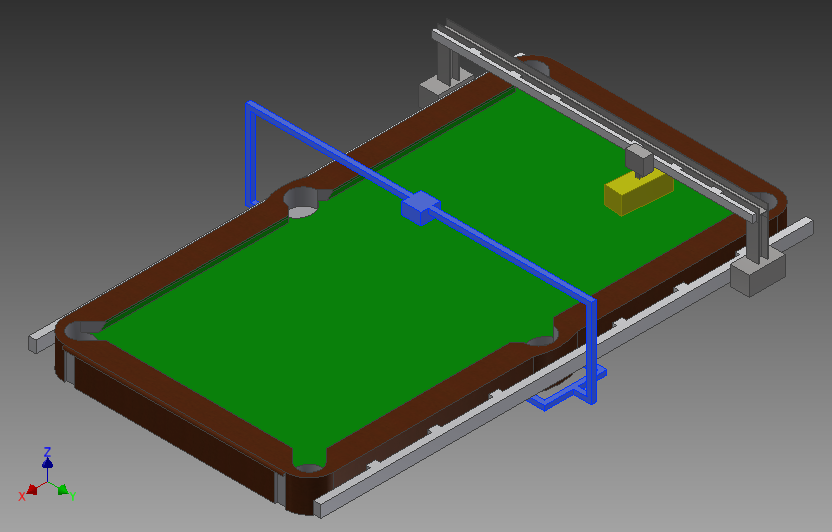
\includegraphics[width = 0.9\textwidth]{cameraMountYAxis.png}
\captionof{figure}{Camera Mount relative to the table (found in blue) } %TODO: add phone holder pic
\label{fig:cameraMount}
\end{center}

\newpage
\subsection{Arm}
\textbf{Description}\\
Extruding vertically from the arm base, the arm connects to the Y-rail and provides stability between the two axes of motion. The arm moves as one with the arm base since they both provide support for the Y Rail.\\~\\
\textbf{Requirements}\\
The arm will be required to remain rigidly perpendicular to the X-rail while supporting its weight (i.e. remain upright without buckling). It is also required to maintain stability when faced with disturbances originating from the end-effector.
\begin{center}
	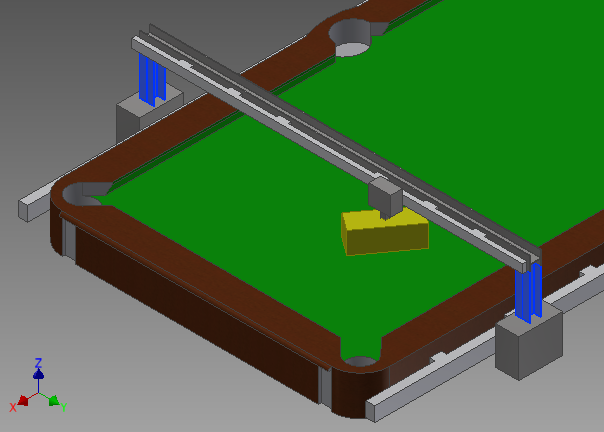
\includegraphics[width = 0.9\textwidth]{arms.png}	% TODO: Include new picture
\captionof{figure}{Arms relative to the table (found in blue)}
\label{fig:armFig}
\end{center}

% TODO: include picture		Arm_base__yrail_exploded.PNG
\subsection{Bracket Connectors to Y Rail}
\textbf{Description}\\
To connect the Y Rail to the Arm L-shaped brackets (displayed in exploded view above) have been used with two connection on both components. These brackets restrict the swinging motion of the rail as it may sway in the y-direction. Once the Arm is stably attached to the X Rail and the Y rail is bolt to the bracket of both sides all motion should be eliminated. It is recommended to bolt the assembly lightly, tune the rails slightly and tighten all bolts to secure connections.\\\\
\textbf{Requirements}\\
The brackets must connect to the Y Rail and Arm in at least two points each per bracket (this is to maintain no unnecessary motion). The bracket must maintain a 90 degree angle between the Arm and the rail as to not apply any bending stresses on either the Arm or the rail. Ensure that the bolts are not interfering with the Y Rail motor or the pulley holder.

% TODO: include picture		Arm_base__arm__xrail_exploded.PNG
\subsection{Timing Belt Holder - X Rail}
\textbf{Description}\\
The Timing Belt Holder (labeled P1 in exploded view) attached to the Arm is used to hold the timing belt and allow for translational motion in the x direction. It is constructed to fit the timing belt tightly so that it may follow the turn of the NEMA 23 motor accurately. This component is 3D printed due to its complex features and sufficient strength.\\\\
\textbf{Requirements}\\
This components is required to hold the belt without slip as to not fail or wear once the motor is moving. It should not apply stress on the belt of drill into the belt since it may cause the belt to fail. Additionally, this belt holder must also be in the direction of the x axis as to maintain a consistent translation of motion from the motor to the Arm. Its height is up to discretion and analysis of the centre of mass.

\subsection{Arm Bolts}
\textbf{Description}\\
The Arm Bolts (labeled B1,2,3,4 in the exploded view) are used to couple the Arm to the Arm Base.\\\\
\textbf{Requirements}\\
These bolts must be flush to the interior face of the Arm Base, as to not interfere with the motion along the rail or hit the Table-Rail Rod Connections (described above).

\subsection{Arm Base}
\textbf{Description}\\
The arm base is a connection between the X-rail and the arm. The arm base is a sturdy component that will move in the X-direction. There are two arm bases, one on each X-rail.\\~\\
\textbf{Requirements}\\
The arm base will be required to move the full length of the X-rail with small amounts of friction. Furthermore, the arm base will be required to support the arm while keeping the arm in a vertical position.
\begin{center}
	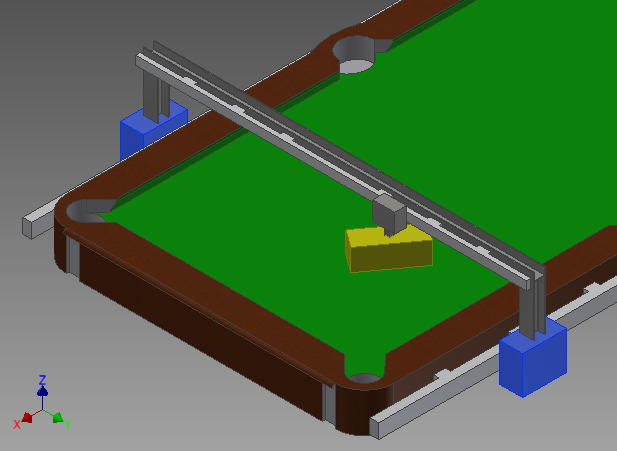
\includegraphics[width = 0.7\textwidth]{armBase.png}	% TODO: Include new picture
\captionof{figure}{Arm Base relative to the table (found in blue)}
\label{fig:armBaseFig}
\end{center}

\subsection{X Rail Wheels}
\textbf{Description}\\
The X Rail Wheels (labeled W1,W2,W3 in exploded view) are the wheels responsible for providing smooth motion along the x direction. The attach to the Arm base with bolts which allow them to spin smoothly. A double nut is placed on either side of the wheels to eliminate their motion along the y direction.\\\\
\textbf{Requirements}\\
The wheels are required to glide along the surface of the X Rail as smoothly as possible to reduce their friction. The wheels must also spin freely along the bolt. Finally, the wheels interior width must be slightly larger than the thickness of the X Rail since it must avoid contact on the sides which result in consistent friction if chosen incorrectly.

% DONE: Just need pics
\subsection{End-Effector}
\textbf{Description}\\
The EE is used to strike the cue ball that is resting on the table. The EE will have rotational capabilities either on its own or along with the EEA.\\~\\
\textbf{Requirements}\\
The EE will be required to accurately provide an impulsive force to the cue ball. Its electromechanical/pneumatic characteristics are further described in the Electromechanical Systems section.
\begin{center}
	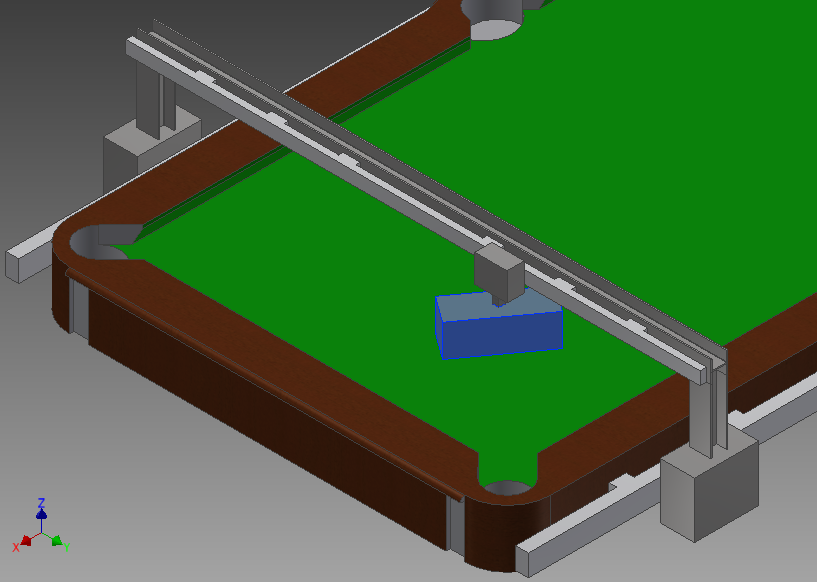
\includegraphics[width = 0.7\textwidth]{endEffector.png}	% TODO: Include standard picture:	sm2_standard.png
\captionof{figure}{End-Effector relative to the table (found in blue)}
\label{fig:eeFig}
\end{center}

% TODO: Include exploded view:	sm2_exploded.png
%\textbf{Description}\\
%Reference End-Effector Arm (EEA) section for detailed description. In this context, the arm will be used to attached components P1 and P2 via nuts.\\~\\
%\textbf{Requirements}\\
%The EEA provides rotational motion and structural support to the End-Effector

\newpage
\subsection{Piston Hinge Connector (P1)}
\textbf{Description}\\
The Piston Hinge Connector (labeled P1 in exploded view) provides a firm connection for the base of the piston. It allows freedom along the axis of rotation necessary for the piston actuation. This part was manufactured using a 3D printer due to its complex features and small size\\~\\
\textbf{Requirements}\\
This component must not restrict the rotary motion of the piston. Additionally, it must reduce the amount of linear freedom along the co-linear direction of bolt B1. This is maintained by reducing the size of the hinge opening as much as possible while still allotting sufficient motion. This component must also be able to move vertically along the EEA in order to tune its location to achieve the best resting height of P3 so that it does not obstruct the ball unnecessarily.

\subsection{Major Hinge Connector (P2)}
\textbf{Description}\\
The Major Hinge Connector (labeled P2 in exploded view) provides a firm connection for component P3 to swing towards the desired ball freely. It allows freedom along the axis of rotation necessary for the P3 component. This part was manufactured using a 3D printer due to its complex features and small size\\~\\
\textbf{Requirements}\\
This component must not restrict the rotary motion of component P3. Additionally, it must reduce the amount of linear freedom along the co-linear direction of bolt B2. This is maintained by reducing the size of the hinge opening as much as possible while still allotting sufficient swinging motion. This component must also be able to move vertically along the EEA in order to tune its location to achieve the best resting height of P3 so that it does not obstruct the ball unnecessarily. Excessive vertical length should be avoided to not obstruct the balls unnecessarily.

\subsection{Striker (P3)}
\textbf{Description}\\
The Striker (labeled P3 in exploded view) is used to make physical contact with the ball. It must be completely solid to avoid wear. The slight angle along its long side is purposed so that the striker piece will strike the balls while perpendicular to the table (this perpendicularity achieves the most ideal shot). The thin protruding connection attaches to the H connector which work together to provide rotational motion. This part was manufactured using a 3D printer due to its complex features and small size (high packing size is recommended).\\~\\
\textbf{Requirements}\\
This component must not restrict the rotary motion of component P3. Additionally, it must reduce the amount of linear freedom along the co-linear direction of bolt B2. This is maintained by reducing the size of the hinge opening as much as possible while still allotting sufficient swinging motion. This component must also be able to move vertically along the EEA in order to tune its location to achieve the best resting height of P3 so that it does not obstruct the ball unnecessarily. Excessive vertical length should be avoided to not obstruct the balls unnecessarily.

\subsection{Piston Hinge (H)}
\textbf{Description}\\
The Psiton Hinge (labeled H in exploded view) which attaches to the tail connection of P3 to convert linear actuation from the piston into rotational motion is P3. The hinge is custom for the specific pneumatic bore size and thread (the corresponding hole size in p3 should be adjusted accordingly).\\~\\
\textbf{Requirements}\\
This component must not restrict the rotary motion of component P3. Additionally, it must reduce the amount of linear freedom along the co-linear direction of its own bolt. This is maintained by increasing the size of P3 as much as possible while still allotting sufficient swinging motion. 

\subsection{Nuts, Bolts and Washers (NBW)}
\textbf{Description}\\
All nuts and bolts should be used according to hole clearance specification provided in schematics. Washers are discouraged in the design of the EE since all mechanical connections are small and should be exact. \\Note: all NBW essential for the description of the system are found in the exploded and standard view but do not show the extent of all NBW required for the system.

\subsection{End-Effector Arm}
\textbf{Description}\\
The End-Effector Arm (EEA) is the connector between the EEB and the EE. It could be a shaft from the motor or a solid piece that is static relative to the EE but rotates in relation to the EEB. The purpose of this component is to lower the height of the EE while providing stability from the Y-rail.\\~\\
\textbf{Requirements}\\
The EEA will be required to remain perpendicular to the surface of the pool table. Furthermore, the EEA will be required to transfer torque to the EE and support the weight of the EE.
\begin{center}
	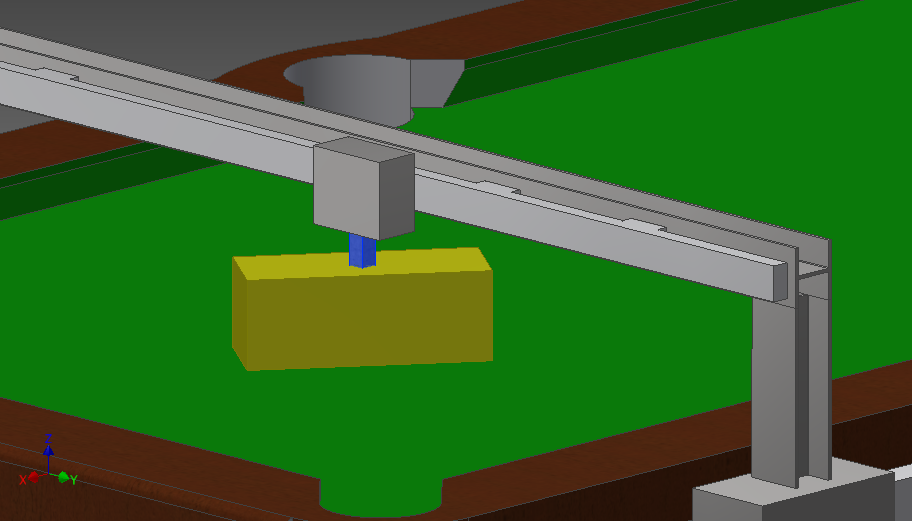
\includegraphics[width = 0.7\textwidth]{efArm.png}	% TODO: Include new picture
\captionof{figure}{End-Effector Arm relative to the table (found in blue)}
\label{fig:eeaFig}
\end{center}

\subsection{End-Effector Base}
\textbf{Description}\\
The End-Effector Base (EEB) supports the EEA and connects it to the Y-rail. It is the connection between the motion of the Y-rail and the EEA. The EEB will likely connect to a belt attached to a motor. It also contains the actuator that provides rotation to the EE through the EEA.\\~\\
\textbf{Requirements}\\
The EEB will be required to move the full length of the Y-rail with a small amount of friction between the Y-rail and itself. Furthermore, the EEB will be required to affix the EEA to the Y-rail. It must also be able to rotate the EEA in order to change the direction of the EE.
\begin{center}
	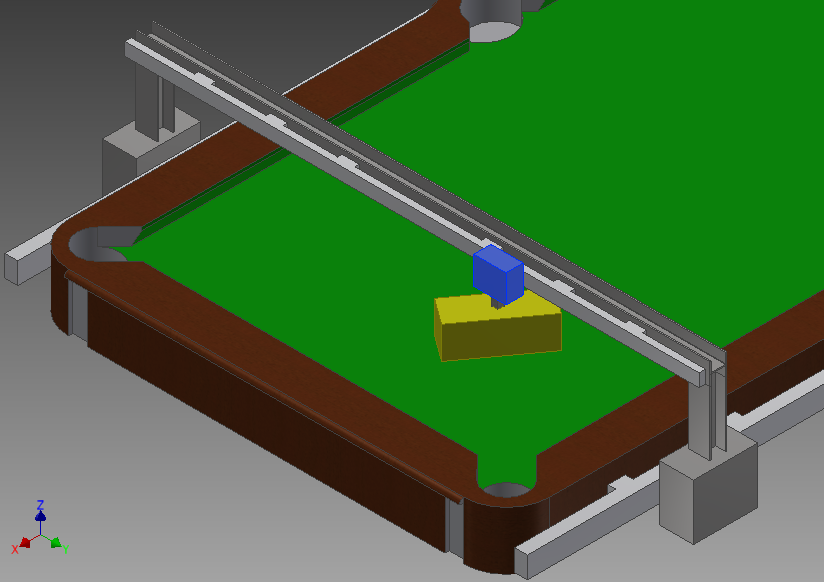
\includegraphics[width = 0.7\textwidth]{efBase.png}	% TODO: Include new picture
\captionof{figure}{End-Effector Base relative to the table (found in blue)}
\label{fig:eebFig}
\end{center}

% TODO: Need to describe components and add pictures
\subsection{Pneumatic system}
\textbf{Description}\\
The Pneumatic system is responsible for providing pneumatic power to the piston used to actuate the shooting mechanism and strike the cue ball. A hydraulic system maybe also be utilized but for simplicity a pneumatic system is chosen.

\subsection{Compressor}
\textbf{Description}\\
The compressor provides compressed air to the pneumatic system which allows for the piston to actuate. The flow rate of the compressor is 32 LPM (somewhat of a limiting factor since the larger this is not fast enough for larger pistons). The compressor is connected to the regulator.\\\\
\textbf{Requirements}\\
The compressor is required to refill the air chamber in order to ensure a consistent pressure for the piston. Once the system is turned on the compressor should also be activated. It must be on for the entire time the system operates or else the system will fail.

\subsection{Regulator}
\textbf{Description}\\
A Pressure Regulator must be integrated in the system which allows the a consistent pressure output from the compressor. The output pressure is variable and should be tuned as the system is tested. In current operation, the pressure is held at 40 PSI for all shots. The input to the regulator is from the compressor and output is to the supply channel of the solenoid valve.\\\\
\textbf{Requirements}\\
The regulator must maintain a consistent output and be easy to tune for the use of the user. 

% TODO: include piston_visual.gif
\subsection{Solenoid Valve (5 way 2 position)}
\textbf{Description}\\
The Solenoid Valve (labeled SV in diagram) is use to manage the airflow of the system. While in its idle state the valve should supply pressure to the retract intake of the piston (closer to the head of the piston). Once the solenoid valve is actuated in its other state it must actuate the extend chamber which allows the piston to move the other components in the shooting mechanism. In order to reduce the noise of the exhaust flow mufflers are used to eliminate noise as much as possible (one muffler for each exhaust, this is optional). The valve is actuated with a 12 volt signal to either solenoid which allows the valve to change state (further described in electromechanical system). \\~\\
\textbf{Requirements}\\
The solenoid valve is required to provide 5 connections without any air leakage and be actuated quickly and accurately as to provide the cylinder with the proper airflow fast.

\subsection{Pneumatic Piston}
\textbf{Description}\\
The Pneumatic Piston (labeled P in diagram) is use to strike the cue ball in the shooting mechanism. Once the piston extends or retracts it moves the striker piece which makes physical contact with the ball. The airflow of the extend and retract chamber are provided from the two outputs of the solenoid valve.\\~\\
\textbf{Requirements}\\
 The dimensions of the of the piston are 1/2 inch bore and 3 inch stroke. These dimensions result from a range of desired specification based on regulator and compressor outputs and availability. The 1/2 inch bore is sufficient when considering a flow rate of 32 LPM. The stroke length is dependant on the arc length of rotation in the striker piece.

\subsection{Piston Fittings}
\textbf{Description}\\
The fittings used for the pneumatic piston are 10/32" push-to-connect fittings. One side is screwed into the piston and sealed using nylon tape while the other connects to tubing (described in tubing section). \\~\\
\textbf{Requirements}\\
The fittings must be snug and now leak any air out of the system. Push-to-fit is recommended but not mandatory. 

\subsection{Tubing}
\textbf{Description}\\
The tubing is plastic and allows for slight flexibility. The outer diameter is partially dependant on the fittings but they may be chosen together so that specific thicknesses can be realized.\\~\\
\textbf{Requirements}\\
The tubing must be flexible enough to not restrict the motion of the system. Its length must be long enough to reach the farthest shot location (for this application a minimum length of 16 ft is required).

\subsection{General Fittings}
\textbf{Description}\\
All tubing connections must be matched to the width of the tube. All connection types in this application are push-to-connect which allows a sealed connection for most standard tubing types. Connections are placed on the regulator, solenoid valve, piston and airflow controller(if necessary).\\~\\
\textbf{Requirements}\\
The threaded connection must be sealed with nylon tape and the valves must not leak air out of the system.

\newpage
\section{Electromechanical System}
This section will go into further detail regarding each electromechanical component that is to be designed as part of this system.
\subsection{X-Rail Motors}
\textbf{Description}\\
As mentioned above, the X rails will traverse the length of the table proving motion in the x-axis. In order to generate this motion, sufficiently strong motors are required to provide power in each direction. There will be two motors due to the width of the table. Both will act synchronously in order to provide equal motion on both sides. The motors will be stepper motors which will allow for accurate measurements of linear distance found through the counting of steps. The motion of the motor will be translated onto the Arm Base through the use of belts or rotational (worm) gears. This allows the motors to remain in one place while the mechanical structure is sliding back and forth (identical belts will be included on both sides). The motors will also be geared in order increase precision and vary the torque applied on the motor.\\~\\
\textbf{Requirements}\\
Based on the specifications of the components moved by the X-rail motor (physical mass, friction, and size of the system) the motor's requirements will be determined. It is imperative that the motor will have enough power to drive the motion. The motor is also required to have a sufficient number of steps in order to track the motion and will be geared accordingly to achieve proper accuracy. Both motors will have the same specifications which will maintain symmetry. 

\subsection{Y-Rail Motor}
\textbf{Description}\\
The Y-rail motor will power the movement required in the Y-direction. Only one motor is needed since the affected components will be supported at a single point on the Y-rail. Similar to the X-rail motors, a stepper motor will be used in order to keep track of the distance traveled along the rail. This motor will be geared as well which will result in a higher resolution of steps and reduce the torque applied on the motor. Additionally, belts will be used in this application as well (similar to the X-Rail Motors) where either a belt or a rotational (worm) gear will be used to translate the rotational motion of the rail gears onto a linear motion in the axis of the y axis.\\~\\
\textbf{Requirements}\\
The electromechanical specifications are reliant on the physical properties of the affected system such as friction coefficients, mass, and size of the components. The motor is also required to have a sufficient number of steps but will be geared if found to require higher accuracy. Finally the motor is required to connect to the motion of the rail either through a belt or another means.

\subsection{Rotational Motor}
\textbf{Description}\\
The Rotational Motor is responsible for properly orienting the EE in the proper direction. It will spin about the axis of the EEA which is attached to the EE at its bottom end. The rotational motor will be housed in the EEB since it provides the most support for a high torque motor. Furthermore, the shaft of the motor will be pointing straight down towards the table to allow the attached EE to reach as close to the table as possible without ball interference. Once the proper orientation is achieved it must remain firmly in place to allow the EE to maintain accuracy whilst attempting a shot. The use of steps or another feedback mechanism will track the current angle of the EE.\\~\\
\textbf{Requirements}\\
The motor is required to spin at least 360 degrees in order to cover all the possible shot angles. The positioning must have a high enough accuracy such that an orientation is achieved within acceptable error. As briefly mentioned in the description section above, the motor must also resist disturbances from the EE to avoid loss of accuracy. Although a stepper motor would be preferred any motor with the ability to track rotational displacement may be used.

\subsection{End-Effector Actuator}
\textbf{Description}\\
The End-Effector (EE) is responsible for striking the cue ball in order to play the game. It is not yet decided whether the actuator will be pneumatic or electromechanical, but either way the final translation of energy to the ball is similar. If pneumatic actuators are chosen then electrical valves will be used to control the flow of air into the pneumatic chamber.\\~\\
\textbf{Requirements}\\
It is very important that the actuator applies sufficient power to the ball so that it can score from all feasible positions on the table. Additionally, in order to direct itself onto the proper orientation it is required to rotate a full 360 degrees. The accuracy of this motion is key to ensuring a proper shot and must be tracked in order to maintain repeatability. The EE must also be easy to maneuver since it is moved by other motors and supported by other structures. Finally, the EE must not interfere with the game/balls in any way, after striking the balls it must allow the balls to roll freely. This works conjointly with the fact that it should take up the least amount of space as possible to increase its workspace.

\newpage
\section{Electrical System}
This section will go into further detail regarding each electrical component that is to be designed as part of this system.
\subsection{Context Diagram}
The following diagram is intended to illustrate the interactions between the electrical components in this system.
\begin{center}
	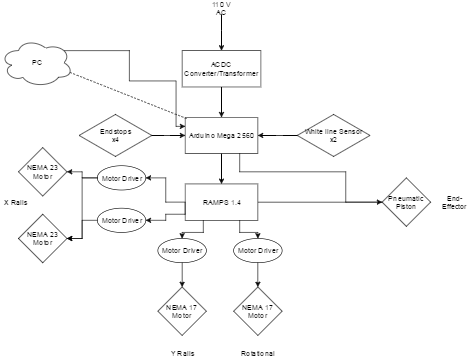
\includegraphics[width = 0.8\textwidth]{ElectricalDiagram.png}
\captionof{figure}{Electrical subsystem context diagram.}
\label{fig:ElectricalDiagramFig}
\end{center}

\newpage
\subsection{List of Electrical Components}
Table \ref{tab:ElectricalComponents} lists all components used in the design of the electrical system.
\begin{table}[h!]
\centering
\caption{Electrical Components}
\begin{tabular}{| p{6cm} | p{6cm} |}\hline
	\textbf{Component}	&\textbf{\centering Quantity}\\\hline
	110V AC Power Supply					&x1\\\hline
	110V AC to 12V DC Converter				&x1\\\hline
	Arduino Mega 2560 $\mu$C				&x1\\\hline
	RAMPS 1.4 Shield						&x1\\\hline
	NEMA 23 Stepper Motor					&x2\\\hline
	NEMA 17 Stepper Motor					&x2\\\hline
	A4988 Stepper Motor Driver				&x4\\\hline
	20-011-968 End Stop					&x4\\\hline
	QRD1114 White Line Sensor				&x2\\\hline
	User Push Button						&x2\\\hline
	Colour Changing LED					&x1\\\hline
	N-type BJT							&x2\\\hline
	Pneumatic Piston						&x1\\\hline
	10K$\Omega$ Resistor					&x2\\\hline
	220$\Omega$ Resistor					&x7\\\hline

\end{tabular}
\label{tab:ElectricalComponents}
\end{table}

\newpage
\subsection{Subsystems}
This subsection depicts detailed designs of the various electrical subsystems that make up the entire electrical system as a whole.

\subsubsection{Push Buttons}
\begin{center}
	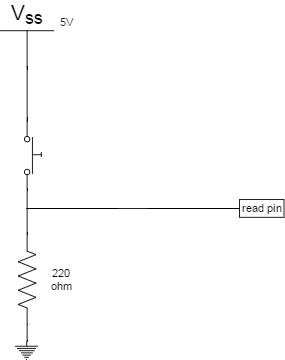
\includegraphics[width = 0.25\textwidth]{PushButton.png}
\captionof{figure}{Push button subsystem.}
\label{fig:PushButtonFig}
\end{center}
\textbf{Description}\\
Pulldown resistor designs are used for the push buttons. When the button is pushed a digital high is read by the $\mu$C, otherwise the $\mu$C reads a digital low.\\\\
\textbf{Components}\\
This subsystem consists of a push button and a 220 $\Omega$ resistor.\\\\
\textbf{Construction}\\
Choose a digital pin on the Arduino Mega 2560 and set it as an INPUT pin in the Arduino code. Then connect a 220 $\Omega$ resistor from the pin to ground. Connect the button to a 5V pin and in parallel to the 220 $\Omega$ resistor.

\subsubsection{Colour Changing LED}
\begin{center}
	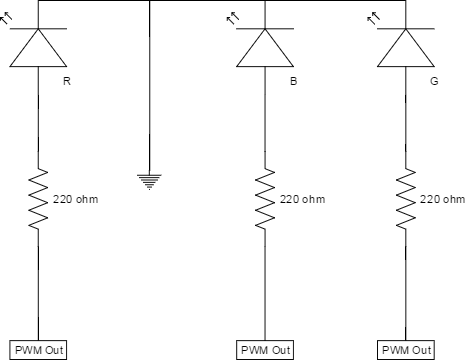
\includegraphics[width = 0.4\textwidth]{ColourChangingLED.png}
\captionof{figure}{Colour changing LED subsystem.}
\label{fig:ColourChangingLEDFig}
\end{center}
\textbf{Description}\\
The $\mu$C uses PWM on the RBG leads of the colour changing LED, and is thereby able to change the colour of light that the LED emits by changing the PWM values at each RBG lead.\\\\
\textbf{Components}\\
This subsystem consists of three 220 $\Omega$ resistors and one colour changing LED bulb.\\\\
\textbf{Construction}\\
Choose three pins capable of PWM (2-13, 44-46)  on the Arduino Mega 2560 and set them as OUTPUT pins. Find the R, B, G and ground leads of the colour changing LED. Connect each of the R,B and G leads in series with a 220 $\Omega$ resistor leading to the respective OUTPUT pins. Connect the ground lead to a ground pin on the Arduino.

\subsubsection{Power Supply to Arduino and RAMPS 1.4}
\begin{center}
	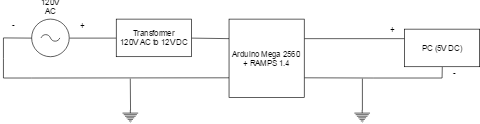
\includegraphics[width = 0.7\textwidth]{PowerSupply.png}
\captionof{figure}{Power supply subsystem.}
\label{fig:PowerSupplyFig}
\end{center}
\textbf{Description}\\
The input voltage of the transformer is 110 AC V from the standard outlet. The transformer/converter reduces this voltage and converts it from AC to 12V DC. The shield is powered by the 12V DC power supply while the arduino is powered by the PC with 5V DC. The transformer has 3 leads from the output - neutral, hot and ground. The transformer has two leads connected to the 12V power component of the shield.\\\\
\textbf{Components}\\
This subsystem consists of a transformer which transforms 110V AC into 12V DC, an Arduino Mega 2560 $\mu$C and a RAMPS 1.4.\\\\
\textbf{Construction}\\
Align the pins of the RAMPS 1.4 with the pins of the Arduino Mega 2560 and then push the two components into each other to form a connection between the two devices. Cut an extension cord open to reveal the three coloured leads inside - black (neutral), green (ground), and red (active). Secure the green wire to the ground inlet of the transformer. Tighten the screw to ensure that the connection is not loose. Secure the red and green wires to the active and neutral inlets, respectively. Use 16 gauge stranded wire to connect the + and - inlets of the transformer to the + and - 12V inlets of the RAMPS 1.4. Tighten the screws on the RAMPS 1.4 to ensure that the connection is not loose. Use the Arduino USB cord to connect the Arduino to a laptop.

\subsubsection{Motors and Motor Drivers}
\begin{center}
	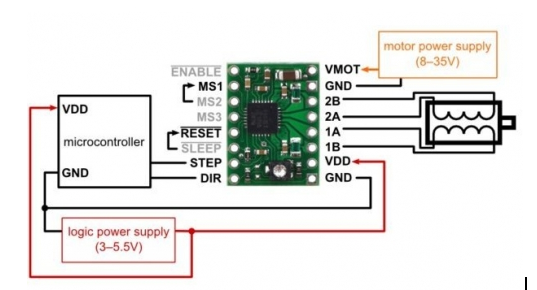
\includegraphics[width = 0.7\textwidth]{Motors.png}
\captionof{figure}{Motor subsystem.}
\label{fig:MotorsFig}
\end{center}
\textbf{Description}\\
The motors will be responsible for generating all motion within the system. They will consist of two motors responsible for moving the end-effector along the length of the table, one motor for moving along the width, and one motor for rotating the end-effector. The motor drivers are an intermediary between the $\mu$C and the motors. The motor dirvers will receive appropriate power from the power supply and control signals (HIGH or LOW) from the $\mu$C. The control signals received from the $\mu$C will govern the performance of the motors. All motors in the system will receive power from their respective motor drivers.\\\\
\textbf{Components}\\
This subsystem consists of an A4988 stepper motor driver, RGB extension wire connecting the four leads from the driver to the motor, and a stepper motor (either NEMA 23 or NEMA 17).\\\\
\textbf{Construction}\\
Connect the A4988 stepper motor driver to the RAMPS 1.4 by connecting the respective pins. Organize the four motor leads in the following order: black, green, red and blue. Extend these leads by connecting them to required length of 16 gauge RGB extension wire. Connect the four leads to the four pins next to the motor driver labeled 2B, 2A, 1A and 1B.

\newpage
\subsubsection{Endstops}
\begin{center}
	\includegraphics[width = 0.6\textwidth]{Endstop.png}
\captionof{figure}{Endstop subsystem.}
\label{fig:elecContextDiagramFig}
\end{center}
\textbf{Description}\\
The endstops are connected to the $\mu$C by three leads - input voltage (5V), ground, and signal. The $\mu$C reads a digital high when the endstop is pushed, and a digital low otherwise. The end-stops will aid in verifying the system's current x and y position.\\\\
\textbf{Components}\\
This system consists of a single endstop sensor.\\\\
\textbf{Construction}\\
The endstop leads can simply be connected to the pins reserved for endstops on the RAMPS 1.4. Ensure that the 5V, ground, and signal leads are connected to their respective pins.

\subsubsection{Pneumatic Piston}
\begin{center}
	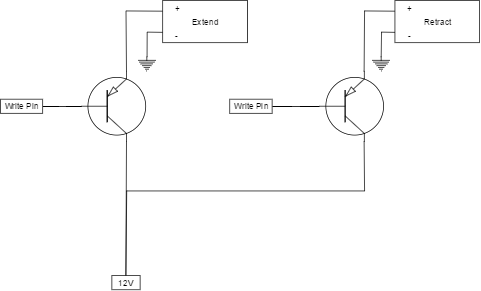
\includegraphics[width = 0.65\textwidth]{PneumaticPiston.png}
\captionof{figure}{Pneumatic piston subsystem.}
\label{fig:PneumaticPistonFig}
\end{center}
\textbf{Description}\\
The pneumatic piston can either be extended or retracted. The extension and retraction motions are powered separately. 12V at 300mA is required per motion. Two n-type BJTs are used to control when the extension or retraction motions occur. When the an output pin sends a high to the BJT gate, the BJT allows current to flow, resulting in the movement of the piston (extension or retraction).\\\\
\textbf{Components}\\
This system consists of a pneumatic piston and two n-type BJTs.\\\\
\textbf{Construction}\\
Find the 12V output inlet on the RAMPS 1.4. Make a connection from this inlet to the emitters of two parallel BJTs. Use two different OUTPUT pins and connect them to the base of the BJTs. Connect each of the collector leads of the BJTs to the positive ends of the pneumatic piston. Connect both of the negative ends to ground.

\subsubsection{Infrared Sensors}
\begin{center}
	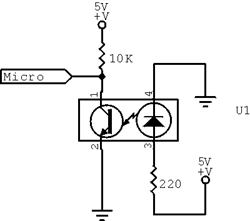
\includegraphics[width = 0.3\textwidth]{IRSensor.png}
\captionof{figure}{ Infrared sensors subsystem.}
\label{fig:IRSensorFig}
\end{center}
\textbf{Description}\\
Two infrared sensors will be integrated in the gear system, one for each gear in the gear train that controls the rotational system. The $\mu$C will read a digital low when the infrared sensors detect the LED light through the small holes in the gear. When both white line sensors read low, the system is oriented in the origin position.\\\\
\textbf{Components}\\
This system consists of a single infrared sensor, a 10 k$\Omega$ resistor and a 220 $\Omega$ resistor.\\\\
\textbf{Construction}\\
Find the leads of the white line sensor labeled 1, 2, 3 and 4, as shown in the figure above.  Connect leads 2 and 4 to ground. Connect lead 3 in series with a 220 $\Omega$ resistor leading into a 5V source. Connect lead 1 to a 10 k$\Omega$ resistor leading to a 5V source. Set up a pin on the Arduino Mega 2560 as an INPUT pin. Connect the INPUT pin from the Arduino Mega 2560 in parallel to the 10 k$\Omega$ resistor.


\end{document}


